\section{Theorie}
\label{sec:Theorie}

In diesem Versuch untersuchen wir den Energietransport zwischen 
zwei Wärmereservoiren, mit dem Ziel die Kenngrößen der 
eingesetzten Wärmepumpe zu ermitteln.

\subsection{Das Prinzip der Wärmepumpe}
Aus Beobachtung von Prozessen in der Natur kann man sagen, dass Wärmeenergie immer vom heißeren zum kälteren
Körper fließt. Durch externe (mechanische) Arbeit kann man diesen Fluß jedoch umkehren. \\
Dabei nimmt nach 
dem ersten Hauptsatz der Wärmelehre das wärmere Reservoir die Wärmeenergie $Q_1$ auf, welche sich aus der
vom kälteren Reservoir entnommenen Wärmemenge $Q_2$, sowie der aufgewandten Arbeit $A$ zusammen:
\begin{equation}
	Q_1 = Q_2 + A
	\label{eqn:waermemenge}
\end{equation}

Davon ausgehend lässt sich die Güteziffer der Wärmepumpe als der Quotient von abgegebener Wärme
und aufgewandter Arbeit definieren:
\begin{equation}
	\nu = \frac{Q_1}{A}
	\label{eqn:gueteziffer}
\end{equation}

Aus dem zweiten Hauptsatz der Thermodynamik lässt sich dabei eine weitere Beziehung herleiten:
Ändert sich die Temperatur zwischen den Reservoiren nicht, so besagt dieser, dass
die Summe der sogenannten 
reduzierten Wärmemengen $\int \frac{\symup{d}Q}{T}$ verschwindet. Dies bedeutet für uns
\begin{equation}
	\frac{Q_1}{T_1} - \frac{Q_2}{T_2} = 0.
	\label{eqn:reduzierte}
\end{equation}

Dabei muss jedoch beachtet werden, dass \eqref{eqn:reduzierte} nur für ideale reversible 
Prozesse gilt. Dies kann von der technischen Realisierung der Wärmepumpe natürlich nicht erreicht werden.
Für den realistischen, irreversiblen Fall gilt die Beziehung
\begin{equation}
	\frac{Q_1}{T_1} - \frac{Q_2}{T_2} > 0.
	\label{eqn:reduzreal}
\end{equation}

Aus den Formeln \ref{eqn:waermemenge} und \ref{eqn:reduzierte} folgt für $Q_1$:
\begin{equation}
	Q_1 = A + \frac{T_2}{T_1} Q_1
	\label{eqn:q1}
\end{equation}

Damit gilt für die in \ref{eqn:gueteziffer} definierte Güteziffer einer idealen Wärmepumpe:
\begin{equation}
	\nu_\text{id} = \frac{Q_1}{A} = \frac{T_1}{T_1 - T_2}
	\label{eqn:gueteideal}
\end{equation}

Beziehungsweise für die Güte einer realen Wärmepumpe gilt
\begin{equation}
	\nu_\text{real} <
	\frac{T_1}{T_1 - T_2}
	\label{eqn:guetereal}
\end{equation}

Mit \ref{eqn:guetereal} lässt sich auch erkennen, dass die Wärmepumpe am effizientesten arbeitet,
wenn die Temperaturdifferenz zwischen den Reservoiren $\vert T_1 - T_2 \vert$ niedrig ist.

\subsection{Die Arbeitsweise der Wärmepumpe}

Die W\"armeenergie wird bei der W\"armepumpe mit einem Gas transportiert, welches beim
Verdunsten W\"arme aus Reservoir 2 aufnimmt und beim Kondensieren an Reservoir 1 abgibt.
\\
Da der Transport aus der Phasenumwandlungsenergie des Gases resultiert, sollte man ein Gas mit einer
m\"oglichst hohen Kondensationsw\"arme benutzen.

\begin{figure}[H]
	\centering
	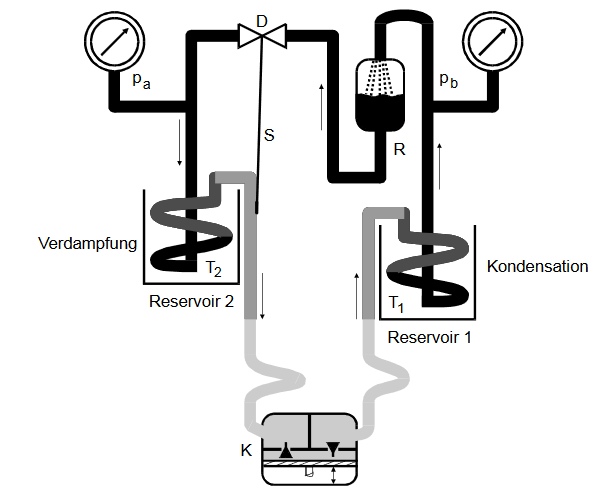
\includegraphics[width=0.9\textwidth]{content/aufbau.jpg}
	\caption{Prinzipieller Aufbau einer W\"armepumpe}
	\cite{anleitung}
	\label{fig:aufbau}
\end{figure}

\autoref{fig:aufbau} zeigt den schematischen Aufbau. Die W\"armepumpe beruht auf einem Kreislauf,
der durch den Kompressor K aufrecht erhalten wird:
\begin{equation}
	\text{Kompressor}
	\rightarrow
	\text{Reservoir 1}
	\rightarrow
	\text{Drosselventil}
	\rightarrow
	\text{Reservoir 2}
	\rightarrow
	\text{Kompressor}
	\rightarrow
	\cdots
	\label{eqn:kreislauf}
\end{equation}
F\"ur den Betrieb der W\"armepumpe soll nun das Gas bei $T_1$ und $p_b$ fl\"ussig und 
bei $T_2$ und $p_a$ gasf\"ormig sein.
\\
Dabei durchl\"uft das Transportmedium folgende Stationen:
\begin{enumerate}
	% Res 1
	\item Das Gas str\"omt vom Kompressor durch Reservoir 1 und kondensiert. Dabei gibt es an
		Res. 1 die Kondeationsw\"arme ab, wodurch Reservoir 1 sich langfristig erw\"armt.
	% Drosselventil
	\item Das nun fl\"ussige Gas flie\ss t durch das Drosselventil D, welches einen Druckunterschied
		$p_b - p_a > 0$ erzeugt.
	% Res 2
	\item Das Fl\"ussiggas str\"omt in Reservoir 2 und wird gassf\"ormig. Die Verdunstung entzieht 
		dabei dem Res. 2 W\"armeenergie, wodurch es abk\"uhlt.
	% Kompressor
	\item Das Gas wird vom Kompressor nahezu adiabatisch komprimmiert.
\end{enumerate}

F\"ur den st\"orungsfreien Betrieb kommen noch weitere Bauteile zum Einsatz, welche jedoch nichts zum
Thermischen Prozess beitragen:
\begin{itemize}
	\item Der Reiniger (In \autoref{fig:aufbau} als ``R`` gekennzeichnet), welcher sicherstellt,
		dass das Fl\"ussiggas keine Luftblasen enth\"alt.
	\item Die Steuervorrichtung ``S``, die sicherstellt, dass keine Fl\"ussigkeitsreste in den 
		Kompressor gelangen, da dieser sonst kaputt gehen w\"urde.
\end{itemize}


\subsection{Die Bestimmung der Kenngrößen einer realen
Wärmepumpe}
\label{sec:bestimmung-kenngroessen}

Bei diesem Versuch interessieren wir uns f\"ur
\begin{itemize}
	\item die G\"uteziffer $\nu$
	\item den Massendurchsatz $\frac{\symup d m}{\symup d t}$
	\item und den Wirkunsgrad des Kompressors  $N_\text{mech}$.
\end{itemize}

\begin{figure}[H]
	\centering
	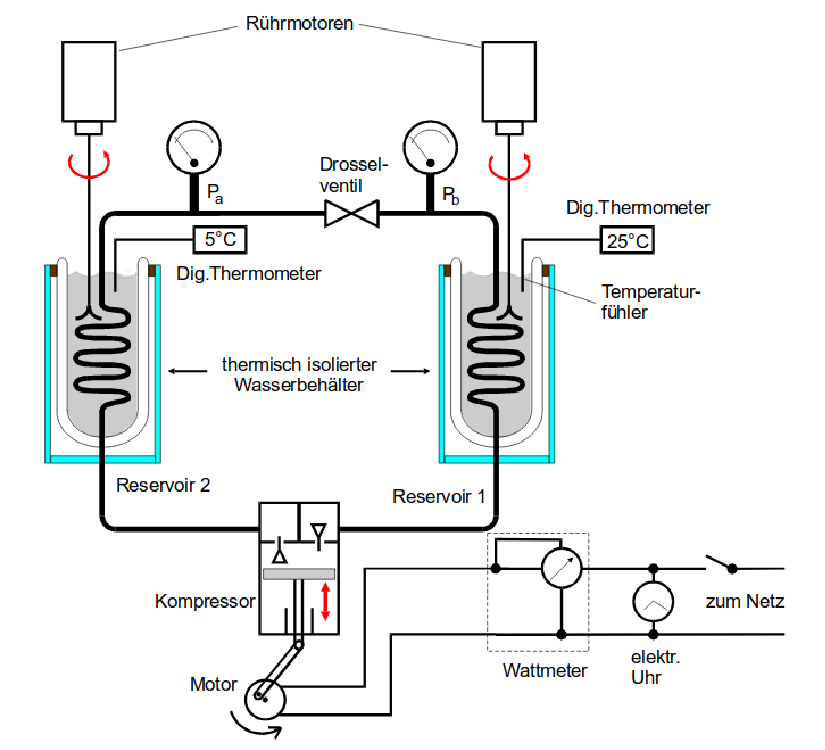
\includegraphics{content/messaperatur.pdf}
	\caption{Schematische Darstellung der kompletten Messaperatur.}
	\cite{anleitung}
	\label{fig:messaperatur}
\end{figure}

Der in \autoref{fig:messaperatur} beschriebene Aufbau erm\"oglicht uns 
die elektrische Leistungsaufnahme des Kompressors,
die Temperaturverl\"aufe in den Reservoiren $T_\text{i}$, 
die Dr\"ucke $p_b$ und $p_a$ (jeweils vor und hinter dem Drosselventil)
in Abh\"angigkeit von der Zeit zu messen.

Die Reservoire wurden hierbei durch zwei isolierte Eimer mit einer genau
definierten Menge Wasser realisiert; um zuverl\"assige Temperaturwerte zu erhalten
werden diese st\"andig umger\"uhrt.

Wenn es gelingt, die Temperaturverl\"aufe als Funktionen der Zeit, also $T_1 = T_1(t)$ und
$T_2 = T_2(t)$ aufzustellen, k\"onnen im nachfolgenden Teil die Differenzenquotienten durch
die entsprechenden Differentialquotienten ersetzt werden.

\subsubsection{Bestimmung der realen Güteziffer}

Aus \ref{eqn:guetereal} wissen wir bereits, dass die Güteziffer der Quotient aus gewonnener Wärme 
$Q_1$ und aufgewandter Arbeit $A$ ist. \\
Für diese Wärmemenge müssen wir zunächst aus der Messreihe $T_1(t)$ für ein geeignetes Intervall 
den Differenzenquotienten $\Delta T_1 / \Delta t$ bilden. Aus diesem ergibt sich dann
\begin{equation}
	\frac{\Delta Q_1}{\Delta t}
	= (m_1 c_\text w + m_\text k c_\text k) \frac{\Delta T_1}{\Delta t},
	\label{eqn:bestgueteziffer1}
\end{equation}
wobei $m_1c_\text w$ der Wärmekapazität des Wassers im Reservoir 1 und $m_\text k c_\text k$ der
Wärmekapazität der Kupferschlange im Eimer entsprechen. Daraus ergibt sich dann die 
Güteziffer
\begin{equation}
	\nu = \frac{\Delta Q_1}{\Delta t \cdot N}
	\label{eqn:messgueteziffer}
\end{equation}
Mit $N$ für die durchschnittliche Kompressorleistung im Zeitintervall $\Delta t$.

\subsubsection{Bestimmung des Massendurchsatzes}

Wie eben für $T_1(t)$ nimmt man ebenfalls den Differenzenquotienten zu $T_2(t)$. Daraus 
ergibt sich dann die pro Zeiteinheit aus Reservoir 2 entnommene Wärmemenge:
\begin{equation}
	\frac{\Delta Q_2}{\Delta t}
	= (m_2 c_\text w + m_\text k c_\text k)  \frac{\Delta T_2}{\Delta t}
	\label{eqn:waermeleitung2}
\end{equation}

Da für die Wärmeentnahme das Transportmedium verdampft und dabei pro Zeit- und Masseneinheit die 
Verdampfungswärme $L$ benötigt wird, gilt der Massendurchsatz
\begin{equation}
	\frac{\Delta m}{\Delta t}
	=
	\frac{1}{L} \frac{\Delta Q_2}{\Delta t}
	\label{eqn:massendurchsatz}
\end{equation}
wenn $L$ bekannt ist.

\subsubsection{Bestimmung der mechanischen Kompressorleistung 
$N_\text{mech}$}

Um ein Gasvolument $V_a$ auf den Wert $V_b$ zu verringern, verrichtet der Kompressor die Arbeit
\begin{equation}
	A_m = 
	-\int_{V_a}^{V_b} p \; \symup{d}V.
	\label{eqn:arbeit-kompresion}
\end{equation}

Als gute N\"aherung nehmen wir nun an, dass die Kompression adiabatisch erfolgt. Dann gilt 
f\"ur den Zusammenhang zwischen Druck und Volumen die bekannte Poissonsche Gleichnug
\begin{equation}
	p_a V_a^\kappa = p_b V_b^\kappa = p V^\kappa
	\label{eqn:poissonsche_Gleichung}
\end{equation}

Dann erhalten wir f\"ur $A_m$
\begin{align}
	A_m 
	&= -p_a V_a^\kappa \int_{V_a}^{V_b} V^{-\kappa} \; \symup dV
	\\
	&= \frac{1}{\kappa - 1} p_a V_a^\kappa \left(V_b^{-\kappa+1} - V_a^{-\kappa +1} \right)
	\\
	&= \frac{1}{\kappa - 1} \left( p_b \sqrt[-\kappa]{\frac{p_a}{p_b}} - p_a \right) V_a
	\label{eqn:a_m}
\end{align}
und f\"ur $N_\text{mech}$
\begin{align}
	N_\text{mech}
	&= \frac{\Delta A_m}{\Delta t}
	\\
	&= \frac{1}{\kappa - 1}  \left( p_b \sqrt[-\kappa]{\frac{p_a}{p_b}} - p_a \right) 
	\frac{\Delta V_a}{\Delta t}
	\\
	&=  \frac{1}{\kappa - 1}  \left( p_b \sqrt[-\kappa]{\frac{p_a}{p_b}} - p_a \right)
	\frac{1}{\rho} \frac{\Delta m}{\Delta t}
	\label{eqn:kompressorleistung}
\end{align}

Hierbei steht $\rho$ f\"ur die Dichte des Transportmediums im gasf\"ormigen Zustand, also 
bei $p = p_a$. Mit der idealen Gasgleichung l\"asst sich $\rho$ aus dem Literaturwert f\"ur
$\rho_0$ unter Normalbedinungen errechnen.
